\chapter{Evaluation}
\label{s:Benchmarks}
Stream fusion is ultimately performed for practical reasons: we want the fused result program to run faster than the original unfused program.
We also need to be sure that the fused program is not too large, otherwise compilation and fusion would consume too much memory.
This chapter shows benchmark results for fused programs and the result size of fused programs.

\section{Benchmarks}

For the benchmarks, I use the Folderol Template Haskell implementation described in \cref{chapter:process:implementation}.
Benchmarks are available at \url{https://github.com/amosr/folderol/tree/master/bench}.
I present one spatial algorithm, two file-based benchmarks, and one audio signal processing benchmark.
The benchmarks are comparing with the array library `Vector', as well as streaming libraries `Conduit', `Pipes' and `Streaming'.

The `Vector' library provides high-performance boxed and unboxed arrays with pull-based shortcut fusion.
It is the \emph{de facto} standard for array programming in Haskell.
While the fusion is pull-based, splits can still be expressed in the program.
When splits are present, they act as fusion barriers, requiring streams to be manifested as in-memory arrays.
Vector also provides no guarantees about whether fusion will occur: it makes its best effort, but the easiest way to tell whether fusion has occurred is to look at the generated program.
We could benchmark the program to see whether it is ``fast enough'', but if we do not have an optimal baseline to compare against, it is hard to know how fast the program \emph{should} be.
After benchmarking, if we discover that fusion has not occurred, it is a completely other thing to convince the compiler to somehow fuse it: perhaps the program must be rewritten and hand-fused, or perhaps strictness annotations are required.

% \TODO{Move elsewhere.}
The Stream part of Vector is split into two types: the fully general stream, which is parameterised over a monad, and pure streams, essentially specialised to the identity monad.
Vector has a minor problem with monadic actions, but this is an implementation detail that could probably be ignored.
Converting from monadic streams back to vectors goes via linked-lists: this is because constructing a vector requires @ST@ or @IO@, but we cannot easily interleave the stream's monadic actions (which may be an arbitrary monad) with effects from @IO@.
Instead, the current implementation runs all of the stream's actions, collecting the result in a list, and only constructs the vector after the stream has finished.
This way, the effects do not need to be interleaved.
It is possible to write this using several unsafe operations, but one must be \emph{very} careful for this, taking into account that laziness must be conquered to ensure the correct interleaving.


The three Haskell streaming libraries, `Conduit', `Pipes', and `Streaming', have a limited API that ensures that any computation can be run with only bounded buffers.
These streaming libraries are pull-based, and do not naturally support multiple outputs: the split in the dataflow graph must be hand-fused, or somehow rewritten as a straight-line computation.
These libraries also have a monadic interface, which allows the structure of the dataflow graph to depend on the values. This expressiveness has a price: if the dataflow graph can change dynamically, we cannot statically fuse it.
% This price is paid even when the dataflow graph is static, as the same monadic structure is used: because repetition is expressed as an unfolding dynamic graph, even computations that would be static in other systems must be expressed dynamically, reducing the possibility for fusion.
If the function that computes the next step of the stream is hidden inside a monadic computation, it is hard for the compiler to pull it out and construct it.
% Why is this? Is this an inherent problem with monadic computations, because the structure of the monad depends dynamically on the input values?
Because the structure --- the function that computes the rest of the stream --- is dynamic, it is hard for the compiler to reason statically about the structure.
In Vector/stream fusion, great effort is taken to make the step function non-recursive and statically known, by splitting the stream into both step function and state.
The step function is completely static, and so can be optimised etc, but the state changes dynamically.
In contrast, in Pipes/Conduit, the step function and state are mixed together: the remainder of the stream is only available dynamically as a function closure, hidden inside a constructor inside a monadic operation.



The benchmark results presented below were all run on a MacBook Pro, with a 2GHz Intel Core i7, and 16GB of RAM.
The operating system is OS X El Capitan.
To run the benchmarks, I used the Criterion\footnote{\url{http://hackage.haskell.org/package/criterion}} library.
Criterion offers a fairly reliable way to evaluate runtime performance, as it runs each benchmark multiple times to compute the mean runtime, and warns if the variance is too high or if there are outliers.
It can also collect statistics on allocations, which is sometimes (but not always) a more stable performance indicator than runtime, as it is less affected by the whims of the underlying operating system.

There are many implementations of the benchmark programs, but for the most part they all follow the same structure.
Showing five different implementations of the same program is not that interesting.
We show the implementations of the Folderol versions; the other versions are available in \cref{app:Benchmarks}.

\subsection{Quickhull}

Quickhull is a divide-and-conquer spatial algorithm to find the smallest convex hull containing all points.
At its core is the @filterMax@ operation which takes a line and an array of points, and finds the farthest point above the line, as well as all points above the line.
The streaming libraries, including Folderol, are parameterised over the monad for effects. For simplicity we use an @IO@ monad.

\begin{lstlisting}[float,label=l:bench:filterMaxFolderol,caption=Folderol implementation of filterMax]
filterMaxFolderol :: Line -> Vector Point -> IO (Point, Vector Point)
filterMaxFolderol l ps = do
  (maxim,(above,())) <- scalar          $ \snkMaxim ->
                        vectorSize   ps $ \snkAbove ->
   $$(fuse $ do
      ins    <- source [|sourceOfVector ps      |]
      annot  <- map    [|\p -> (p, distance p l)|] ins
      above  <- filter [|\(_,d) -> d > 0        |] annot
      above' <- map    [|fst                    |] above
      maxim  <- maxBy  [|compare `on` snd       |] annot
      sink maxim       [|snkMaxim               |]
      sink above'      [|snkAbove               |]$$)
  return (fst maxim, above)
\end{lstlisting}

\Cref{l:bench:filterMaxFolderol} shows the Folderol implementation of @filterMax@.
The Folderol implementation starts by constructing a sink for the maximum point to be pushed into (@snkMaxim@), and a sink for the vector of points above the line (@snkAbove@).
As we know the output vector of points is not going to be any longer than the input vector, we use @vectorSize@ as a size hint to remove the need to dynamically grow the vector (\cref{s:implementation:sizehints}).
The Template Haskell splice calls @fuse@ to convert the process network into executable code.
The process network starts by converting the input vector @pts@ to a stream @ins@.
We use @source@ to create an input stream, which takes a Template Haskell expression denoting how to construct a source at runtime.
We then annotate each point of @ins@ with the distance between each point and the line with @map@, calling this stream @annot@.
The @annot@ stream is filtered to only those above the line (@above@), then the annotations thrown away (@above'@).
The maximum is computed by comparing the second half of each annotated point --- the distance --- and stored in @maxim@.
Finally, @maxim@ is pushed into the scalar output sink, and all @above'@ points are pushed into the vector output sink.


Let us now look at two versions of @filterMax@ using Vector.
The shortcut fusion system cannot fuse both operations into a single loop, and both operations require the distances between the line and each point.
This means a choice must be made: either compute the distances upfront and share them, or recompute the distances in each operation.
I compare both implementations.

\begin{lstlisting}[float,label=l:bench:filterMaxVectorShare,caption=Vector / share implementation of filterMax]
filterMaxVectorShare l ps
 = let annot = map (\p -> (p, distance p l)) ps
       point = fst
             $ maximumBy (compare `on` snd) annot
       above = map fst
             $ filter ((>0) . snd) annot
   in return (point, above)
\end{lstlisting}

The shared distances implementation is shown in \cref{l:bench:filterMaxVectorShare}.
First, compute the distance between each point and the line, and store this in a vector called @annot@.
Then @point@ computes the maximum with @maximumBy@, comparing each distance.
Next, @above@ filters each point.

The recomputed distances implementation is available in \cref{app:Benchmarks}, \cref{l:a:bench:filterMaxVectorRecompute}.
To recompute the vectors, we start from the shared version and duplicate the @annot@ vector to @annot1@ and @annot2@. The maximum now uses @annot1@, and filter uses @annot2@.
This way, both maps to compute the distance can be fused into their consumers.

In the results below, recomputing the distances is faster than storing the distances.
For this benchmark we used only two-dimensional points, but it is possible that at higher dimensions the cost of recomputing distances may outweigh the cost of allocation.
Also, the choice to recompute the distances requires intimate knowledge of how shortcut fusion works and might be surprising to the naive user: duplicating work does not usually \emph{improve} performance.

For Conduit, we also have two versions: the first uses two passes over the data, while the second is hand-fused into a single loop.
The two-pass version defines two `conduits', or stream computations; @cabove@ for the filtered vector and @cmaxim@ for the maximum.
Computation @cabove@ converts the vector to a conduit with @sourceVector@, then annotates with the distances, filters according to the distances, removes the annotations, and converts back to a vector.
As with Folderol, we use size hints when converting back to a vector to remove any overhead with growing and copying the vector.
Computation @cmaxim@ also converts the vector to a conduit, then annotates with the distances, and computes the maximum.
The hand-fused Conduit version is more complicated, and loses the abstraction benefits from using a high-level streaming library.

For Pipes, we only have a hand-fused version, which follows much the same structure as the Conduit hand-fused version.

Finally, the Streaming version is much closer to the Vector version, except that the stream must be explicitly split into both consumers.
We start by converting the vector to a stream with @sourceVector@, and then use @map@ to annotate each point with the distance from the line.
To split the stream, we use @store@ which takes a computation to perform on the copy of the stream --- in this case computing the maximum with @maximumBy@.
The original stream is also passed through, which is filtered and then the annotations discarded.

\begin{table}
\begin{center}
\begin{tabular}{ll|rrrr}
& & Runtime (s)  & Runtime (\%) & Allocation (b) & Allocation (\%) \\
\hline
Folderol &          & 0.21s &   100\% & 1.2e9 & 100\% \\
Hand     &          & 0.14s &    66\% & 4.8e8 &  40\% \\
&&&\\
Vector & store      & 0.40s &   190\% & 1.8e9 & 150\%\\
       & recompute  & 0.34s &   161\% & 8.0e8 & 66\%\\
&&&\\
Conduit & 2-pass    & 10.0s & 4,762\% & 6.2e10& 5,167\% \\
       & hand       &  7.9s & 3,762\% & 4.4e10& 3,667\% \\
&&&\\
Pipes  & hand       &  4.9s & 1,876\% & 3.9e10& 3,250\% \\
Streaming &         &  4.4s & 2,095\% & 3.0e10& 2,500\% \\
\end{tabular}
\end{center}
\caption[Quickhull benchmark results]{Quickhull benchmark results}
\label{table:bench:quickhull}
\end{table}

\Cref{table:bench:quickhull} shows the runtimes for Quickhull over $10^7$ points, which corresponds to around 150MB in memory.
Different sizes of data produce similar results.
The hand-fused version is the fastest, followed by Folderol.
The Vector versions are somewhat slower because they require two iterations over the data, but still generate high-quality loops.
Intimate knowledge of shortcut fusion was required to find `recompute', the faster of the two vector benchmarks, and there is no indication in the source program, or from the compiler, that the two could not be fused together.
The streaming libraries are significantly slower, spending most of the time allocating closures and forcing thunks.
Why are they so much slower? This would be better in the motivation.
On the plus side, the limited APIs and linearity constraints for Conduit and Pipes made it more obvious that they would not be fused into a single loop, but even with partial hand-fusion, are still significantly slower.
The `Streaming' program allows explicit sharing, and was the simplest of the three streaming libraries, requiring no hand fusion.
Surprisingly, the simpler `Streaming' program is faster than the hand-fused `Conduit' and `Pipes' programs, but is still significantly slower than Folderol.

It would be nice to know why the Folderol version is slower than the hand-fused version.
Inspecting the assembly, the code is very similar.
The difference between hand-fused and Folderol appears to be that the Folderol implementation is spilling sixteen more bytes to the stack every iteration.

These streaming libraries are not usually used for array computations because of this overhead.
In practice, one tends to `chunk' the data so that each element is an array of multiple elements: this reduces overhead paid for streaming.
This chunking complicates the program further, again reducing the level of abstraction the programmer can work at.
Even with chunking, we may reduce the streaming overhead from once per element to once per thousand elements, but we can never remove it entirely.
With Folderol there is no streaming overhead to reduce because it is statically fused away.

\subsection{Dynamic range compression}
Dynamic range compression is an audio signal processing algorithm to reduce the volume of loud sounds, leaving quiet sounds unchanged.
To implement this, we take an audio signal, and at each point compute a rolling average of the volume.
We clip the volume at the upper bound, one, and divide the clipped volume by the original volume.
This will be our multiplier, which we multiply the original signal by at each step.
This way, if the volume is less than the limit, our multiplier will be one and the signal is unchanged. 
If the volume is above the limit, our multiplier will be the reciprocal of volume: whatever is required to get the volume back down to one.

\begin{lstlisting}[float,label=l:bench:compressorFolderol,caption=Folderol implementation of compressor]
compressor :: Vector Double -> IO (Vector Double)
compressor vecIns = do
  (vecOut,()) <- vectorSize vecIns $ \snkOut -> do
    $$(fuse $ do
        ins     <- source    [|sourceOfVector vecIns|]
        squares <- map       [|\x -> x * x|]       ins
        avg     <- postscanl [|lop        |] [|0|] squares
        mul     <- map       [|clip       |]       avg
        out     <- zipWith   [|(*)        |] mul   ins
        sink out             [|snkOut     |]$$)
  return vecOut
 where
  lop acc sample = acc * 0.9 + sample * 0.1

  clip mean
   = let root    = sqrt mean
     in  min 1.0 root / root
\end{lstlisting}

The Folderol version is shown in \cref{l:bench:compressorFolderol}.
To implement this in Folderol, we start by creating a sink for our output vector, calling the sink @snkOut@ and the vector @vecOut@.
This will be the same size as the input vector, so we use @vectorSize@.
We take the input array @vecIns@ and convert it to a stream @ins@.
We are going to compute the volume of the input stream using the \emph{root mean square}, so first we need to square each element.
This is the @squares@ stream.
We need to compute the average of the squares, so we will use an exponential moving average --- which is equivalent to as a low-pass filter.
To compute the moving average, we use @postscanl@, which is like a fold over the data, except it returns the stream of accumulators rather than just the final result.
The difference between @postscanl@ and regular @scanl@ is that the output stream for @scanl@ contains the original zero accumulator for the fold, while @postscanl@ omits this.
Now that we have our average, @avg@, we @clip@ each element by taking the square root, and clipping it to one. This is our multiplier, @mul@.
Finally, we zip the original stream with the multiplier, and multiply them together.

The Vector version is very similar to the Folderol version, except without the Template Haskell boilerplate.
The shortcut fusion \emph{is} able to fuse this into a single loop, except the two occurrences of the input vector mean that it will be indexed twice.

\Cref{table:bench:compressor} shows the runtimes for the dynamic range compressor over $10^8$ samples, which corresponds to around 750MB in memory.
The difference between the hand-fused version and the Folderol version are very slight, and may be due to operating system scheduling overhead. 
The Vector version is slower because its generated loop indexes the input array twice.

\begin{table}
\begin{center}
\begin{tabular}{ll|rrrr}
& & Runtime (s)  & Runtime (\%) & Allocation (b) & Allocation (\%) \\
\hline
Folderol &          & 0.93s &   100\% & 8.0e8 & 100\% \\
Hand     &          & 0.98s &   105\% & 8.0e8 & 100\% \\
&&&\\
Vector &            & 1.78s &   191\% & 8.0e8 & 100\%\\
\end{tabular}
\end{center}
\caption[Compressor benchmark results]{Compressor benchmark results}
\label{table:bench:compressor}
\end{table}

\subsection{Dynamic range compression with low-pass}
Before compressing an audio signal, we may wish to perform some pre-processing on it.
For this example, suppose we want to apply a low-pass filter to the input signal.

\begin{lstlisting}[float,label=l:bench:compressorLopFolderol,caption=Folderol implementation of compressor with low-pass]
compressorLop :: Vector Double -> IO (Vector Double)
compressorLop vecIns = do
  (vecOut,()) <- vectorSize vecIns $ \snkOut -> do
    $$(fuse $ do
        ins     <- source    [|sourceOfVector vecIns|]
        lopped  <- postscanl [|lop20k     |] [|0|] ins
        squares <- map       [|\x -> x * x|]       lopped
        avg     <- postscanl [|lop        |] [|0|] squares
        mul     <- map       [|clip       |]       avg
        out     <- zipWith   [|(*)        |] mul   lopped
        sink out             [|snkOut     |]$$)
  return vecOut
\end{lstlisting}

The code for compressor with a low-pass is shown in \cref{l:bench:compressorLopFolderol}.
Here we again use @postscanl@ to create another low-pass filter, calling the result @lopped@.
Then @lopped@ is used as the input to both @squares@ and @out@.

\begin{table}
\begin{center}
\begin{tabular}{ll|rrrr}
& & Runtime (s)  & Runtime (\%) & Allocation (b) & Allocation (\%) \\
\hline
Folderol &          & 1.16s &   100\% & 8.0e8 & 100\% \\
Hand     &          & 1.18s &   101\% & 8.0e8 & 100\% \\
&&&\\
Vector &            & 2.21s &   190\% & 1.6e9 & 200\%\\
\end{tabular}
\end{center}
\caption[Compressor with low-pass benchmark results]{Compressor with low-pass benchmark results}
\label{table:bench:compressorlop}
\end{table}

\Cref{table:bench:compressorlop} shows the results for compressor with low-pass.
For the Vector implementation, in the previous example the two occurrences of @ins@ just meant that the input array was indexed twice.
However, in the modified version it is not an input vector being used twice, but the result of @postscanl@.
This means that the result vector for @lopped@ must be reified into a manifest vector, before it can be reused.
The Vector version then has two loops, as well as an extra manifest array.





\subsection{File operations}
For the file benchmarks, we compare against three Haskell streaming libraries: `Conduit', `Pipes', and `Streaming'.
These streaming libraries are pull-based, and do not naturally support multiple outputs: the split in the dataflow graph must be hand-fused, or somehow rewritten as a straight-line computation.
These libraries also have a monadic interface, which allows the structure of the dataflow graph to depend on the values. This expressiveness has a price: if the dataflow graph can change dynamically, we cannot statically fuse it.
% This price is paid even when the dataflow graph is static, as the same monadic structure is used: because repetition is expressed as an unfolding dynamic graph, even computations that would be static in other systems must be expressed dynamically, reducing the possibility for fusion.

\begin{lstlisting}[float,label=l:bench:append2Folderol,caption=Folderol implementation of append2]
append2 :: FilePath -> FilePath -> FilePath -> IO Int
append2 fpIn1 fpIn2 fpOut = do
  (count,()) <- scalarIO $ \snkCount ->
    $$(fuse $ do
      in1   <- source [|sourceLinesOfFile fpIn1|]
      in2   <- source [|sourceLinesOfFile fpIn2|]
      aps   <- append in1 in2
      count <- fold   [|\c _ -> c + 1|] [|0|] aps

      sink count      [|snkCount               |]
      sink aps        [|sinkFileOfLines fpOut  |]$$)
  return count
\end{lstlisting}

\begin{lstlisting}[float,label=l:bench:part2Folderol,caption=Folderol implementation of part2]
part2 :: FilePath -> FilePath -> FilePath -> IO (Int, Int)
part2 fpIn1 fpOut1 fpOut2 = do
  (c1,(c2,())) <- scalarIO $ \snkC1 -> scalarIO $ \snkC2 ->
    $$(fuse defaultFuseOptions $ do
      in1       <- source    [|sourceLinesOfFile fpIn1|]
      (o1s,o2s) <- partition [|\l -> length l `mod` 2 == 0|] in1

      c1        <- fold      [|\c _ -> c + 1|] [|0|] o1s
      c2        <- fold      [|\c _ -> c + 1|] [|0|] o2s

      sink c1                [|snkC1                 |]
      sink c2                [|snkC2                 |]
      sink o1s               [|sinkFileOfLines fpOut1|]
      sink o2s               [|sinkFileOfLines fpOut2|]$$)
  return (c1, c2)
\end{lstlisting}

The first file benchmark simply appends two files while counting the lines.
In Pipes and Conduit, counting the lines is implemented as a pipe which counts each line before passing it along.
\Cref{table:bench:append2} shows the runtimes for appending two text files each with half a million lines, around 6.5MB in total.



\begin{table}
\begin{center}
\begin{tabular}{ll|rrrr}
& & Runtime (s)  & Runtime (\%) & Allocation (b) & Allocation (\%) \\
\hline
Folderol &          & 0.29s &   100\% & 8.6e8 & 100\% \\
Hand     &          & 0.29s &   100\% & 8.6e8 & 100\% \\
Conduit &           & 0.93s &   320\% & 3.3e9 & 383\% \\
Pipes  &            & 0.94s &   324\% & 3.4e9 & 395\% \\
Streaming &         & 0.57s &   196\% & 2.6e9 & 302\% \\
\end{tabular}
\end{center}
\caption[Append2 benchmark results]{Append2 benchmark results}
\label{table:bench:append2}
\end{table}

The second file benchmark takes a file and partitions it into two files: one with even-length lines, and one with odd-length lines.
The output lines are also counted.
Even with partial hand-fusion because of the multiple outputs, the Pipes and Conduit programs are slower than ours, as well as losing the abstraction benefits from using a high-level library.
The `Streaming' library allows streams to be shared in a fairly straightforward way and does not require hand-fusion, but is also the slowest in this benchmark.
\Cref{table:bench:part2} shows the runtimes for partitioning a file with one million lines, around 6.5MB.

\begin{table}
\begin{center}
\begin{tabular}{ll|rrrr}
& & Runtime (s)  & Runtime (\%) & Allocation (b) & Allocation (\%) \\
\hline
Folderol &          & 0.30s &   100\% & 8.6e8 & 100\% \\
Hand     &          & 0.30s &   100\% & 8.6e8 & 100\% \\
Conduit & hand      & 0.66s &   220\% & 2.4e9 & 279\% \\
Pipes  & hand       & 0.55s &   183\% & 2.0e9 & 232\% \\
Streaming &         & 1.21s &   403\% & 6.1e9 & 709\% \\
\end{tabular}
\end{center}
\caption[Part2 benchmark results]{Part2 benchmark results}
\label{table:bench:part2}
\end{table}

\subsection{Partition / append}

\begin{lstlisting}[float,label=l:bench:partitionAppendFail,caption=Partition / append fusion failure]
partitionAppendFailure :: Vector Int -> IO (Vector Int)
partitionAppendFailure xs = do
  (ys,()) <- vectorSize xs $ \snkYs ->
    $$(fuse $ do
        x0    <- source [|sourceOfVector xs|]
        as    <- filter [|even             |] x0
        bs    <- filter [|odd              |] x0
        -- Failure: cannot fuse append with both filters
        asbs  <- append as bs
        sink asbs       [|snkYs            |]$$)
  return ys
\end{lstlisting}

If we try to compile the code in \cref{l:bench:partitionAppendFail}, we get a compilation error:
\begin{code}
Maximum process count exceeded:
 after fusion there are 2 processes, but maximum is 1
\end{code}
This indicates that the program could not be fused into a single loop, without introducing unbounded buffering.
This is because @append@ requires all the @as@ first: all the even-valued elements need to be read from the stream, before the odd-valued elements can be read by append.
But this means that when reading from the stream, if we see an odd-valued element, we would need to hold on to it until we were sure there were no even-valued elements left.

In this case, the input stream is not really a stream, but is backed by a real vector.
So we can actually implement it without introducing an unbounded buffer: we already have the buffer.
To execute the program, we \emph{explicitly} introduce another source to read from the vector. 
See \cref{l:bench:partitionAppend2Source}.
The two filters now apply to different input sources, even though they are backed by the same vector, so there is no need to coordinate the two uses.
All of @as@ can be read by @append@, independently of @bs@.

\begin{lstlisting}[float,label=l:bench:partitionAppend2Source,caption=Partition / append with two sources]
partitionAppend2Source xs = do
  (ys,()) <- vectorSize xs $ \snkYs ->
    $$(fuse $ do
        x0    <- source [|sourceOfVector xs|]
        x1    <- source [|sourceOfVector xs|]
        as    <- filter [|even             |] x0
        bs    <- filter [|odd              |] x1
        asbs  <- append as bs
        sink asbs       [|snkYs            |]$$)
  return ys
\end{lstlisting}

But we can actually implement it another way, if we are willing to introduce two intermediate arrays.
In this version we introduce two loops.
In the first loop, we partition the input into two intermediate arrays.
Then in the second loop, we append the two intermediate arrays.
See \cref{l:bench:partitionAppend2Loop}.

\begin{lstlisting}[float,label=l:bench:partitionAppend2Loop,caption=Partition / append with two loops]
partitionAppend2Loop xs = do
  (as,(bs,())) <- vectorSize xs $ \snkAs ->
                  vectorSize xs $ \snkBs ->
    $$(fuse $ do
        x0      <- source    [|sourceOfVector xs|]
        (as,bs) <- partition [|even             |] x0
        sink as              [|snkAs            |]
        sink bs              [|snkBs            |]$$)
  (ys,()) <- vectorSize xs $ \snkYs ->
    $$(fuse $ do
        as'   <- source      [|sourceOfVector as|]
        bs'   <- source      [|sourceOfVector bs|]
        asbs  <- append as' bs'
        sink asbs            [|snkYs            |]$$)
  return ys
\end{lstlisting}

\begin{table}
\begin{center}
\begin{tabular}{ll|rrrr}
& & Runtime (s)  & Runtime (\%) & Allocation (b) & Allocation (\%) \\
\hline
Folderol & 2-loop   & 0.17s &   100\% & 2.4e8 & 100\% \\
         & 2-source & 0.28s &   165\% & 8.0e7 &  33\% \\
Vector   & 2-loop   & 0.15s &    88\% & 1.6e8 &  67\% \\
         & 2-source & 0.26s &   153\% & 1.6e8 &  67\% \\
\end{tabular}
\end{center}
\caption[PartitionAppend2 benchmark results]{PartitionAppend2 benchmark results}
\label{table:bench:part2app2}
\end{table}

\Cref{table:bench:part2app2} shows the runtimes for partitioning and appending an input file with $10^7$ lines.

The Vector implementations follow the same structure: the 2-loop version uses an intermediate array to store the filtered arrays in before appending them; the other indexes the input array twice, thus computing the predicate twice.
Note that the 2-loop Vector version uses the @partition@ primitive, which is itself a hand-fused implementation of two filters.
The Vector @partition@ cannot fuse with any consumers and always constructs manifest output vectors.
The fact that it constructs a manifest vector does allow an optimisation that Folderol cannot perform: if the size is known, the output can be filled at both ends, with the true parts filling the start of the array, and the false parts filling from the back of the array.
The length of both partitions must equal the length of the original array.
Once the end is reached, the false parts which were filled backwards can be reversed in-place.
Unfortunately, the Vector program still splits this array in two and appends it back together: which should be the same as not splitting the array in the first place.

In the table, the Vector version with two loops is the fastest, but the difference between it and Folderol with two loops is fairly small.
The Folderol version with two sources uses the least memory - a third of the two loop Folderol, and a half of the Vector versions.
Sometimes, we are willing to sacrifice lower throughput for lower memory usage, and this decision really depends on the context.
So by giving a compilation error when fusion fails, we are able to maintain a high level of abstraction, while at the same time forcing the author to make these scheduling decisions.
The author must explicitly choose when is the right time to reuse an array, when is the right time to introduce a new loop, and when is the right time to introduce intermediate buffers.
This way, the result of fusion should not be magic or surprising.
The author can be confident that if it compiles, it will have the desired streaming behaviour.

% -----------------------------------------------------------------------------
\section{Result Size}
% \TODO{Update with Folderol sizes}

As with any practical fusion system, we must be careful that the size of the result code does not become too large when more and more processes are fused together.
\Cref{fig:bench:outputsize} shows the maximum number of output states in the result when a particular number of processes are fused together in a pipelined-manner.
To produce this graph we programmatically generated dataflow networks for \emph{all possible} pipelined combinations of the @map@, @filter@, @scan@, @group@ and @merge@ combinators, and tried all possible fusion orders consiting of adjacent pairs of processes.
The @merge@ combinator itself has two inputs, so only works at the very start of the pipeline --- we present result for pipelines with and without a @merge@ at the start.
The same graph shows the number of states in the result when the various combinations of combinators are fused in parallel, for example, we might have a @map@ and a @filter@ processing the same input stream.
In both cases the number of states in the result process grows linearly with the number of processes. In all combinations, with up to 7 processes there are fewer than 100 states in the result process. 

The size of the result process is roughly what one would get when inlining the definitions of each of the original source processes. This is common with other systems based on inlining and/or template meta-programming, and is not prohibitive.

On the other hand, \cref{fig:bench:exponential} shows the results for a pathological case where the size of the output program is exponential in the number of input processes. The source dataflow networks consists of N merge processes, N+1 input streams, and a single output stream. The output of each merge process is the input of the next, forming a chain of merges. In source notation the network for N = 3 is @sOut = merge sIn1 (merge sIn2 (merge sIn3 sIn4))@.

When fusing two processes the fusion algorithm essentially compares every state in the first process with every state in the second, computing a cross product. During the fusion transform, as states in the result process are generated they are added to a finite map --- the @instrs@ field of the process definition. The use of the finite map ensures that identical states are always combined, but genuinely different states always make it into the result. 

In the worst case, fusion of two processes produces O($n*m$) different states, where $n$ and $m$ are the number of states in each. If we assume the two processes have about the same number of states then this is O($n^2$). Fusing the next process into this result yields O($n^3$), so overall the worst case number of states in the result will be O($n^k$), where $k$ is the number of processes fused. 

In the particular case of @merge@, the implementation has two occurrences of the @push@ instruction. During fusion, the states for the consuming process are inlined at each occurrence of @push@. These states are legitimately different because at each occurence of @push@ the input channels of the merge process are in different channel states, and these channel states are included in the overall process state.




% -----------------------------------------------------------------------------
\begin{figure}
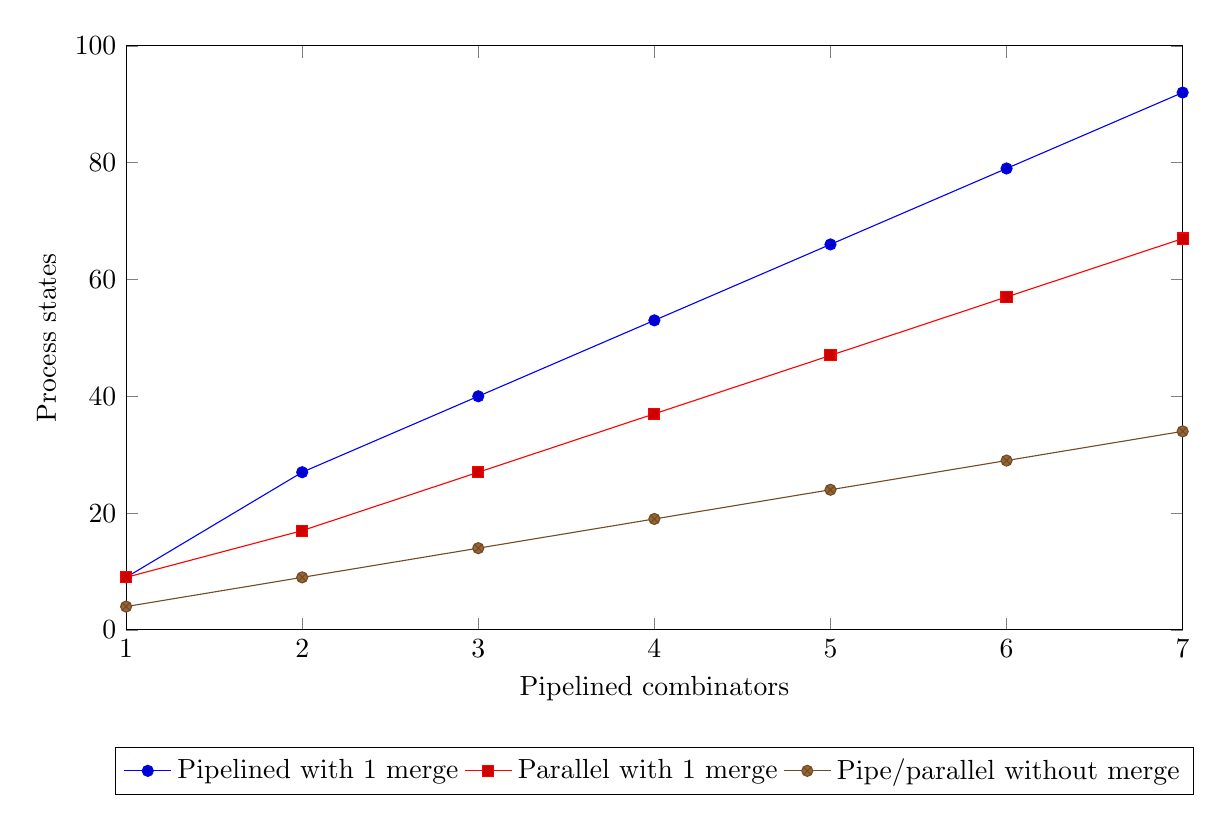
\begin{tikzpicture}
\begin{axis}[
% Hide the label on the second graph
	ylabel=Process states,
	xlabel=Pipelined combinators,
  ymin=0, ymax=100,
  xmin=1, xmax=7,
  xtick=data,
    width=15cm, height=9.0cm,
    legend style={at={(0.5,-0.2)},anchor=north, legend columns=4},
]
\addplot coordinates {(1,9) (2,27) (3,40) (4,53) (5,66) (6,79) (7,92) };
\addplot coordinates {(1,9) (2,17) (3,27) (4,37) (5,47) (6,57) (7,67) };
\addplot coordinates {(1,4) (2,9) (3,14) (4,19) (5,24) (6,29) (7,34)  };

\legend{Pipelined with 1 merge, Parallel with 1 merge, Pipe/parallel without merge};
\end{axis}
\end{tikzpicture}

\caption{Maximum output process size for fusing all combinations of up to $n$ combinators.}
\label{fig:bench:outputsize}
\end{figure}


% -----------------------------------------------------------------------------
\begin{figure}

\begin{tikzpicture}
\begin{axis}[
	ylabel=Process states,
	xlabel=Number of merges,
%  ymode=log,
  ymin=0, ymax=1500,
	enlargelimits=0.01,
  xtick=data,
  xmin=1, xmax=7,
    width=15cm, height=9.0cm,
	legend pos=north west,
]
% These are the values for splitting.
% They are smaller than the 'chaining', but look much nicer on the linear graph.
\addplot coordinates {(1,9) (2,42) (3,97) (4,196) (5,383) (6,746) (7,1461) (8,2880) };

% These are the values for chaining
% \addplot coordinates {(1,4) (2,48) (3,194) (4,760) (5,2814) (6,10064) (7,1) };

\end{axis}
\end{tikzpicture}

\caption{Exponential blowup occurs when splitting or chaining merges together.}
\label{fig:bench:exponential}
\end{figure}



\section{Conclusion}
In the benchmarks, we saw that Folderol was always competitive with the hand-fused program, and in all but a few cases, faster than the other programs.
For array computations there is a bit of boilerplate required to convert between vectors and streams, and vice versa.
There is also some extra visual noise for the Template Haskell.
But this is fairly minor, and the required changes are more or less mechanical and type-driven.

The real benefit is not having to read through Core programs, not having to guess whether fusion has worked or failed.
If fusion succeeds, we know it has succeeded.
If fusion fails, we know not just that it has failed, but \emph{where} it has failed.
It is a lot easier to track down the failure.

